
%% bare_conf.tex
%% V1.3
%% 2007/01/11
%% by Michael Shell
%% See:
%% http://www.michaelshell.org/
%% for current contact information.
%%
%% This is a skeleton file demonstrating the use of IEEEtran.cls
%% (requires IEEEtran.cls version 1.7 or later) with an IEEE conference paper.
%%
%% Support sites:
%% http://www.michaelshell.org/tex/ieeetran/
%% http://www.ctan.org/tex-archive/macros/latex/contrib/IEEEtran/
%% and
%% http://www.ieee.org/

%%*************************************************************************
%% Legal Notice:
%% This code is offered as-is without any warranty either expressed or
%% implied; without even the implied warranty of MERCHANTABILITY or
%% FITNESS FOR A PARTICULAR PURPOSE! 
%% User assumes all risk.
%% In no event shall IEEE or any contributor to this code be liable for
%% any damages or losses, including, but not limited to, incidental,
%% consequential, or any other damages, resulting from the use or misuse
%% of any information contained here.
%%
%% All comments are the opinions of their respective authors and are not
%% necessarily endorsed by the IEEE.
%%
%% This work is distributed under the LaTeX Project Public License (LPPL)
%% ( http://www.latex-project.org/ ) version 1.3, and may be freely used,
%% distributed and modified. A copy of the LPPL, version 1.3, is included
%% in the base LaTeX documentation of all distributions of LaTeX released
%% 2003/12/01 or later.
%% Retain all contribution notices and credits.
%% ** Modified files should be clearly indicated as such, including  **
%% ** renaming them and changing author support contact information. **
%%
%% File list of work: IEEEtran.cls, IEEEtran_HOWTO.pdf, bare_adv.tex,
%%                    bare_conf.tex, bare_jrnl.tex, bare_jrnl_compsoc.tex
%%*************************************************************************

% *** Authors should verify (and, if needed, correct) their LaTeX system  ***
% *** with the testflow diagnostic prior to trusting their LaTeX platform ***
% *** with production work. IEEE's font choices can trigger bugs that do  ***
% *** not appear when using other class files.                            ***
% The testflow support page is at:
% http://www.michaelshell.org/tex/testflow/



% Note that the a4paper option is mainly intended so that authors in
% countries using A4 can easily print to A4 and see how their papers will
% look in print - the typesetting of the document will not typically be
% affected with changes in paper size (but the bottom and side margins will).
% Use the testflow package mentioned above to verify correct handling of
% both paper sizes by the user's LaTeX system.
%
% Also note that the "draftcls" or "draftclsnofoot", not "draft", option
% should be used if it is desired that the figures are to be displayed in
% draft mode.
%
\documentclass[10pt, conference, compsocconf]{IEEEtran}
% Add the compsocconf option for Computer Society conferences.
%
% If IEEEtran.cls has not been installed into the LaTeX system files,
% manually specify the path to it like:
% \documentclass[conference]{../sty/IEEEtran}





% Some very useful LaTeX packages include:
% (uncomment the ones you want to load)


% *** MISC UTILITY PACKAGES ***
%
%\usepackage{ifpdf}
% Heiko Oberdiek's ifpdf.sty is very useful if you need conditional
% compilation based on whether the output is pdf or dvi.
% usage:
% \ifpdf
%   % pdf code
% \else
%   % dvi code
% \fi
% The latest version of ifpdf.sty can be obtained from:
% http://www.ctan.org/tex-archive/macros/latex/contrib/oberdiek/
% Also, note that IEEEtran.cls V1.7 and later provides a builtin
% \ifCLASSINFOpdf conditional that works the same way.
% When switching from latex to pdflatex and vice-versa, the compiler may
% have to be run twice to clear warning/error messages.






% *** CITATION PACKAGES ***
%
%\usepackage{cite}
% cite.sty was written by Donald Arseneau
% V1.6 and later of IEEEtran pre-defines the format of the cite.sty package
% \cite{} output to follow that of IEEE. Loading the cite package will
% result in citation numbers being automatically sorted and properly
% "compressed/ranged". e.g., [1], [9], [2], [7], [5], [6] without using
% cite.sty will become [1], [2], [5]--[7], [9] using cite.sty. cite.sty's
% \cite will automatically add leading space, if needed. Use cite.sty's
% noadjust option (cite.sty V3.8 and later) if you want to turn this off.
% cite.sty is already installed on most LaTeX systems. Be sure and use
% version 4.0 (2003-05-27) and later if using hyperref.sty. cite.sty does
% not currently provide for hyperlinked citations.
% The latest version can be obtained at:
% http://www.ctan.org/tex-archive/macros/latex/contrib/cite/
% The documentation is contained in the cite.sty file itself.






% *** GRAPHICS RELATED PACKAGES ***
%
\ifCLASSINFOpdf
  % \usepackage[pdftex]{graphicx}
  % declare the path(s) where your graphic files are
  % \graphicspath{{../pdf/}{../jpeg/}}
  % and their extensions so you won't have to specify these with
  % every instance of \includegraphics
  % \DeclareGraphicsExtensions{.pdf,.jpeg,.png}
\else
  % or other class option (dvipsone, dvipdf, if not using dvips). graphicx
  % will default to the driver specified in the system graphics.cfg if no
  % driver is specified.
  % \usepackage[dvips]{graphicx}
  % declare the path(s) where your graphic files are
  % \graphicspath{{../eps/}}
  % and their extensions so you won't have to specify these with
  % every instance of \includegraphics
  % \DeclareGraphicsExtensions{.eps}
\fi
% graphicx was written by David Carlisle and Sebastian Rahtz. It is
% required if you want graphics, photos, etc. graphicx.sty is already
% installed on most LaTeX systems. The latest version and documentation can
% be obtained at: 
% http://www.ctan.org/tex-archive/macros/latex/required/graphics/
% Another good source of documentation is "Using Imported Graphics in
% LaTeX2e" by Keith Reckdahl which can be found as epslatex.ps or
% epslatex.pdf at: http://www.ctan.org/tex-archive/info/
%
% latex, and pdflatex in dvi mode, support graphics in encapsulated
% postscript (.eps) format. pdflatex in pdf mode supports graphics
% in .pdf, .jpeg, .png and .mps (metapost) formats. Users should ensure
% that all non-photo figures use a vector format (.eps, .pdf, .mps) and
% not a bitmapped formats (.jpeg, .png). IEEE frowns on bitmapped formats
% which can result in "jaggedy"/blurry rendering of lines and letters as
% well as large increases in file sizes.
%
% You can find documentation about the pdfTeX application at:
% http://www.tug.org/applications/pdftex





% *** MATH PACKAGES ***
%
%\usepackage[cmex10]{amsmath}
% A popular package from the American Mathematical Society that provides
% many useful and powerful commands for dealing with mathematics. If using
% it, be sure to load this package with the cmex10 option to ensure that
% only type 1 fonts will utilized at all point sizes. Without this option,
% it is possible that some math symbols, particularly those within
% footnotes, will be rendered in bitmap form which will result in a
% document that can not be IEEE Xplore compliant!
%
% Also, note that the amsmath package sets \interdisplaylinepenalty to 10000
% thus preventing page breaks from occurring within multiline equations. Use:
%\interdisplaylinepenalty=2500
% after loading amsmath to restore such page breaks as IEEEtran.cls normally
% does. amsmath.sty is already installed on most LaTeX systems. The latest
% version and documentation can be obtained at:
% http://www.ctan.org/tex-archive/macros/latex/required/amslatex/math/





% *** SPECIALIZED LIST PACKAGES ***
%
%\usepackage{algorithmic}
% algorithmic.sty was written by Peter Williams and Rogerio Brito.
% This package provides an algorithmic environment fo describing algorithms.
% You can use the algorithmic environment in-text or within a figure
% environment to provide for a floating algorithm. Do NOT use the algorithm
% floating environment provided by algorithm.sty (by the same authors) or
% algorithm2e.sty (by Christophe Fiorio) as IEEE does not use dedicated
% algorithm float types and packages that provide these will not provide
% correct IEEE style captions. The latest version and documentation of
% algorithmic.sty can be obtained at:
% http://www.ctan.org/tex-archive/macros/latex/contrib/algorithms/
% There is also a support site at:
% http://algorithms.berlios.de/index.html
% Also of interest may be the (relatively newer and more customizable)
% algorithmicx.sty package by Szasz Janos:
% http://www.ctan.org/tex-archive/macros/latex/contrib/algorithmicx/




% *** ALIGNMENT PACKAGES ***
%
%\usepackage{array}
% Frank Mittelbach's and David Carlisle's array.sty patches and improves
% the standard LaTeX2e array and tabular environments to provide better
% appearance and additional user controls. As the default LaTeX2e table
% generation code is lacking to the point of almost being broken with
% respect to the quality of the end results, all users are strongly
% advised to use an enhanced (at the very least that provided by array.sty)
% set of table tools. array.sty is already installed on most systems. The
% latest version and documentation can be obtained at:
% http://www.ctan.org/tex-archive/macros/latex/required/tools/


%\usepackage{mdwmath}
%\usepackage{mdwtab}
% Also highly recommended is Mark Wooding's extremely powerful MDW tools,
% especially mdwmath.sty and mdwtab.sty which are used to format equations
% and tables, respectively. The MDWtools set is already installed on most
% LaTeX systems. The lastest version and documentation is available at:
% http://www.ctan.org/tex-archive/macros/latex/contrib/mdwtools/


% IEEEtran contains the IEEEeqnarray family of commands that can be used to
% generate multiline equations as well as matrices, tables, etc., of high
% quality.


%\usepackage{eqparbox}
% Also of notable interest is Scott Pakin's eqparbox package for creating
% (automatically sized) equal width boxes - aka "natural width parboxes".
% Available at:
% http://www.ctan.org/tex-archive/macros/latex/contrib/eqparbox/





% *** SUBFIGURE PACKAGES ***
%\usepackage[tight,footnotesize]{subfigure}
% subfigure.sty was written by Steven Douglas Cochran. This package makes it
% easy to put subfigures in your figures. e.g., "Figure 1a and 1b". For IEEE
% work, it is a good idea to load it with the tight package option to reduce
% the amount of white space around the subfigures. subfigure.sty is already
% installed on most LaTeX systems. The latest version and documentation can
% be obtained at:
% http://www.ctan.org/tex-archive/obsolete/macros/latex/contrib/subfigure/
% subfigure.sty has been superceeded by subfig.sty.



%\usepackage[caption=false]{caption}
%\usepackage[font=footnotesize]{subfig}
% subfig.sty, also written by Steven Douglas Cochran, is the modern
% replacement for subfigure.sty. However, subfig.sty requires and
% automatically loads Axel Sommerfeldt's caption.sty which will override
% IEEEtran.cls handling of captions and this will result in nonIEEE style
% figure/table captions. To prevent this problem, be sure and preload
% caption.sty with its "caption=false" package option. This is will preserve
% IEEEtran.cls handing of captions. Version 1.3 (2005/06/28) and later 
% (recommended due to many improvements over 1.2) of subfig.sty supports
% the caption=false option directly:
%\usepackage[caption=false,font=footnotesize]{subfig}
%
% The latest version and documentation can be obtained at:
% http://www.ctan.org/tex-archive/macros/latex/contrib/subfig/
% The latest version and documentation of caption.sty can be obtained at:
% http://www.ctan.org/tex-archive/macros/latex/contrib/caption/




% *** FLOAT PACKAGES ***
%
%\usepackage{fixltx2e}
% fixltx2e, the successor to the earlier fix2col.sty, was written by
% Frank Mittelbach and David Carlisle. This package corrects a few problems
% in the LaTeX2e kernel, the most notable of which is that in current
% LaTeX2e releases, the ordering of single and double column floats is not
% guaranteed to be preserved. Thus, an unpatched LaTeX2e can allow a
% single column figure to be placed prior to an earlier double column
% figure. The latest version and documentation can be found at:
% http://www.ctan.org/tex-archive/macros/latex/base/



%\usepackage{stfloats}
% stfloats.sty was written by Sigitas Tolusis. This package gives LaTeX2e
% the ability to do double column floats at the bottom of the page as well
% as the top. (e.g., "\begin{figure*}[!b]" is not normally possible in
% LaTeX2e). It also provides a command:
%\fnbelowfloat
% to enable the placement of footnotes below bottom floats (the standard
% LaTeX2e kernel puts them above bottom floats). This is an invasive package
% which rewrites many portions of the LaTeX2e float routines. It may not work
% with other packages that modify the LaTeX2e float routines. The latest
% version and documentation can be obtained at:
% http://www.ctan.org/tex-archive/macros/latex/contrib/sttools/
% Documentation is contained in the stfloats.sty comments as well as in the
% presfull.pdf file. Do not use the stfloats baselinefloat ability as IEEE
% does not allow \baselineskip to stretch. Authors submitting work to the
% IEEE should note that IEEE rarely uses double column equations and
% that authors should try to avoid such use. Do not be tempted to use the
% cuted.sty or midfloat.sty packages (also by Sigitas Tolusis) as IEEE does
% not format its papers in such ways.





% *** PDF, URL AND HYPERLINK PACKAGES ***
%
%\usepackage{url}
% url.sty was written by Donald Arseneau. It provides better support for
% handling and breaking URLs. url.sty is already installed on most LaTeX
% systems. The latest version can be obtained at:
% http://www.ctan.org/tex-archive/macros/latex/contrib/misc/
% Read the url.sty source comments for usage information. Basically,
% \url{my_url_here}.





% *** Do not adjust lengths that control margins, column widths, etc. ***
% *** Do not use packages that alter fonts (such as pslatex).         ***
% There should be no need to do such things with IEEEtran.cls V1.6 and later.
% (Unless specifically asked to do so by the journal or conference you plan
% to submit to, of course. )


% correct bad hyphenation here
\usepackage{graphicx}
\usepackage{booktabs} % Para bordas bonitas
\usepackage{multirow} % Para células que ocupam múltiplas linhas
\usepackage{siunitx} % Para alinhar números com incertezas
\usepackage{hyperref}
\usepackage{graphicx}
\sisetup{
  separate-uncertainty=true, % Habilita o formato "x ± y"
  table-align-uncertainty=true, % Alinha corretamente incertezas na tabela
}
\hyphenation{op-tical net-works semi-conduc-tor}
\begin{document}
%
% paper title
% can use linebreaks \\ within to get better formatting as desired
\title{A detecção precoce de patologias cardiovasculares}


% author names and affiliations
% use a multiple column layout for up to two different
% affiliations

\author{\IEEEauthorblockN{Nome: Guilherme Fernandes Rezende Santos}
\IEEEauthorblockA{RA: 813467}
}

% conference papers do not typically use \thanks and this command
% is locked out in conference mode. If really needed, such as for
% the acknowledgment of grants, issue a \IEEEoverridecommandlockouts
% after \documentclass

% for over three affiliations, or if they all won't fit within the width
% of the page, use this alternative format:
% 
%\author{\IEEEauthorblockN{Michael Shell\IEEEauthorrefmark{1},
%Homer Simpson\IEEEauthorrefmark{2},
%James Kirk\IEEEauthorrefmark{3}, 
%Montgomery Scott\IEEEauthorrefmark{3} and
%Eldon Tyrell\IEEEauthorrefmark{4}}
%\IEEEauthorblockA{\IEEEauthorrefmark{1}School of Electrical and Computer Engineering\\
%Georgia Institute of Technology,
%Atlanta, Georgia 30332--0250\\ Email: see http://www.michaelshell.org/contact.html}
%\IEEEauthorblockA{\IEEEauthorrefmark{2}Twentieth Century Fox, Springfield, USA\\
%Email: homer@thesimpsons.com}
%\IEEEauthorblockA{\IEEEauthorrefmark{3}Starfleet Academy, San Francisco, California 96678-2391\\
%Telephone: (800) 555--1212, Fax: (888) 555--1212}
%\IEEEauthorblockA{\IEEEauthorrefmark{4}Tyrell Inc., 123 Replicant Street, Los Angeles, California 90210--4321}}




% use for special paper notices
%\IEEEspecialpapernotice{(Invited Paper)}




% make the title area
\maketitle

\textbf{\textit{Resumo} - A detecção precoce de patologias cardiovasculares é crucial na medicina pediátrica, uma vez que muitas dessas condições se desenvolvem de forma assintomática 
até estágios avançados. A identificação precoce pode melhorar significativamente o prognóstico e permitir tratamentos mais eficazes. Recentemente, avanços tecnológicos, incluindo o uso de 
aprendizado de máquina (AM), têm contribuído para aprimorar estratégias de diagnóstico, permitindo a análise eficiente de grandes volumes de dados médicos e auxiliando na tomada de 
decisão clínica. Este projeto utiliza uma base de dados real coletada no Real Hospital Português (RHP), no Brasil, referência em atendimento pediátrico e pioneiro na adoção de tecnologias 
de análise de dados para monitoramento cardiovascular.}


\section{Introdução}
A detecção precoce de patologias cardiovasculares em pacientes pediátricos é um tema de crescente importância na medicina, uma vez que essas condições podem se desenvolver de 
forma assintomática durante a infância e adolescência, muitas vezes só sendo identificadas em estágios avançados. As doenças cardiovasculares são a principal causa de morte no mundo, 
com aproximadamente 17,9 milhões de mortes em 2016, sendo que 17 milhões dessas mortes ocorreram de forma prematura, antes dos 70 anos de idade (OrganizaçãoPan-Americana de Saúde, 2016)\footnote{\href{https://www.paho.org/pt/topicos/doencas-cardiovasculares}{OPAN - Doenças cardiovasculares}}. 

A identificação precoce dessas patologias não apenas melhora o prognóstico dos pacientes, mas também possibilita a implementação de tratamentos preventivos mais eficazes, o que pode 
prevenir complicações graves e salvar vidas. A evolução das tecnologias de monitoramento e diagnóstico, aliada ao uso de ferramentas de aprendizado de máquina, tem revolucionado a forma 
como doenças cardiovasculares são diagnosticadas e tratadas em crianças e jovens. Em particular, o uso de dados clínicos coletados em ambientes hospitalares tem se mostrado uma estratégia 
poderosa para identificar padrões e fatores preditivos de doenças cardíacas em populações pediátricas. 

A análise desses dados, que incluem informações como pressão arterial, índice de
massa corporal, entre outros parâmetros vitais, oferece uma visão mais clara da saúde cardiovascular de crianças, permitindo a antecipação de tratamentos. Além disso, o uso de algoritmos 
de aprendizado de máquina para análise desses grandes volumes de dados tem mostrado resultados promissores na melhoria da precisão dos diagnósticos e na personalização dos cuidados 
médicos. 

A partir dessa perspectiva, o projeto visa desenvolver um sistema de detecção precoce de patologias cardiovasculares em pacientes pediátricos 
utilizando diferentes técnicas de aprendizado de máquina. O sistema será treinado e validado com a base de dados coletada no Real Hospital Português (RHP), visando identificar padrões 
e fatores de risco que possam indicar a presença de doenças cardíacas. A implementação desses modelos poderá auxiliar os profissionais de saúde na tomada de decisões clínicas 
mais informadas e na adoção de medidas preventivas, contribuindo para a melhoria da qualidade de vida e do prognóstico dos pacientes.

\section{Trabalhos relacionados}
O conjunto de dados fornecidos possui diversas colunas categóricas, o que torna necessário mapear esses dados para valores numéricos, a fim de 
possibilitar o uso dos dados para treinamento do modelo. Em Aprendizado de Máquina para Predição de Diagnósticos de Doenças Cardiovasculares,
Francisco Romes da Silva Filho e Emanuel F. Coutinho.(2022)\cite{IEEEhowto:kopka}, houve uma situação semelhante, na qual foi utilizado o método 
multi-hot encoding para a transformação dos dados. Com base nessa escolha, surgiu a ideia de aplicar o método one-hot encoding para transformar os dados.

Segundo o estudo sobre as consequências da DCV.Ghosh et al. (2021) \cite{citekey}, foi demonstrada a eficácia do método de classificação Random Forest para a 
classificação de doenças cardíacas, o que abriu a possibilidade de utilizar o mesmo modelo neste projeto.



\section{Análise de dados e pré-processamento}
O dataset foi desenvolvido pelo Real Hospital Português (RHP) com o objetivo de facilitar o estudo e a identificação de padrões 
associados a doenças cardiovasculares. O conjunto de dados é composto por um arquivo extenso no formato .csv, no qual cada 
linha corresponde a uma amostra distinta.

Cada amostra representa um paciente único que realizou uma consulta cardiológica e é caracterizada por 20 atributos, 
descritos a seguir:
\begin{itemize}
  \item Peso do paciente em Kg.
  \item Altura do paciente em cm.
  \item IMC (índice de massa corporal) do paciente.
  \item Atendimento: data da consulta.
  \item DN: data de escrita da declaração de nascido vivo do paciente.
  \item Idade do paciente.
  \item Convênio do paciente.
  \item Pulsos: atributo categórico que indica a qualidade da circulação arterial do cliente.
  \item Pressão Arterial Sistólica (PA SISTOLICA): valor mais alto em mmHg que aparece durante uma aferição de pressão.
  \item Pressão Arterial Diastólica (PA DIASTOLICA): valor mais baixo em mmHg que aparece durante uma aferição de pressão.
  \item PPA (Pressão Pulso Arterial): atributo categórico que descreve o estado da pressão arterial de um paciente com base em medições clínicas.
  \item B2 (Segundo Ruído Cardíaco): atributo categórico que representa o estado do som de fechamento das válvulas aórticas e pulmonar.
  \item Sopro: atributo categórico que está relacionado à ausculta cardíaca e descreve a presença e características de sopros no coração.
  \item Frequência Cardíaca (FC) do paciente medidos em batimentos por minuto (bpm).
  \item HDA1 (Histórico de doenças atual 1): representa o  primeiro problema clínico do histórico do paciente.
  \item HDA2 (Histórico de doenças atual 2): representa o segundo problema clínico do histórico do paciente. 
  \item Genêro biológico do paciente.
  \item Motivo 1: primeira razão para a consulta.
  \item Motivo 2: segunda razão para a consulta.
\end{itemize}

\vspace{0.3cm}

\subsection{Preparação dos dados}
O conjunto de dados contém dados de treino e dados de teste juntos, sendo cada um deles identificado pelo Id da amostra. Como os dados de teste
não possuem a classe da amostra, não podem ser utilizados durante o processo de treinamento dos modelos. Levando isso em conta, separamos os dados do
dataset RHP.csv em dois outros sub-conjuntos:

\begin{itemize}
  \item train-data: contém as amostras utilizadas para treinamento dos modelos.
  \item test-data: contém as amostras utilizadas para as predições no Kaggle.
\end{itemize}

\vspace{0.3cm}

\subsection{Análise dos dados}
A análise dos dados foi conduzida por meio da visualização e interpretação de gráficos, os quais relacionam os atributos 
com a classe alvo. Para os atributos categóricos, foram utilizados gráficos de barras, que 
permitem visualizar a distribuição das diferentes categorias de cada atributo em relação à classe. 
No caso dos atributos numéricos, optou-se por gráficos boxplot, que possibilitam a análise da distribuição dos valores e sua 
dispersão em relação à classe.

Após a análise dos gráficos, pode-se obter um planejamento do que deveria ser realizado no pré-processamento, 
identificando a necessidade de transformações específicas nos dados. Por exemplo, a presença de valores irreais em 
atributos numéricos pode demandar imputação, enquanto a existência de valores redundantes ou inconsistentes em colunas 
categóricas pode requerer a padronização desses valores. Além disso, para atributos categóricos com múltiplas categorias, 
é essencial aplicar técnicas como o one-hot encoding.
\begin{figure}[htbp]
  \centering
  \begin{minipage}{0.2\textwidth} 
    \centering
    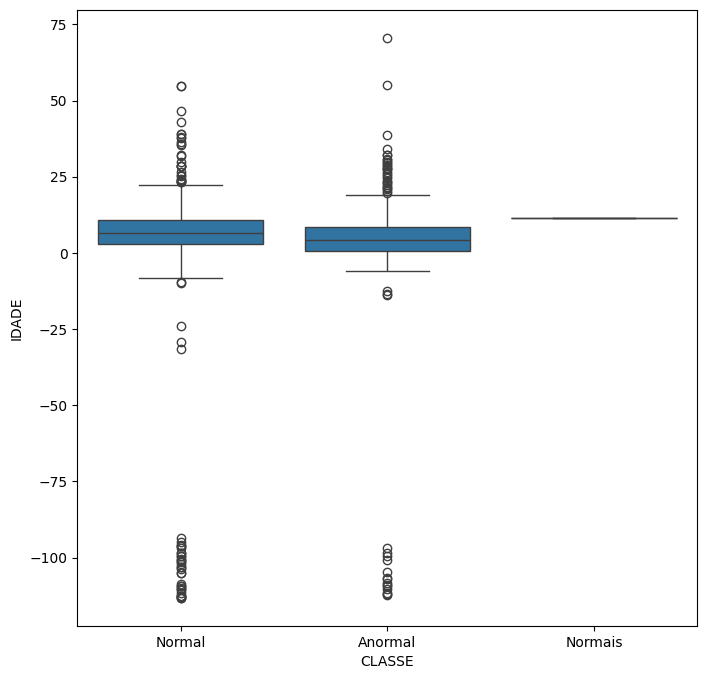
\includegraphics[width=\textwidth]{box_plot_idade.png} 
    \tiny{\caption{Box plot da idade}}
    \label{fig:box_plot_idade}
  \end{minipage}
  \hfill 
  \begin{minipage}{0.2\textwidth}
    \centering
    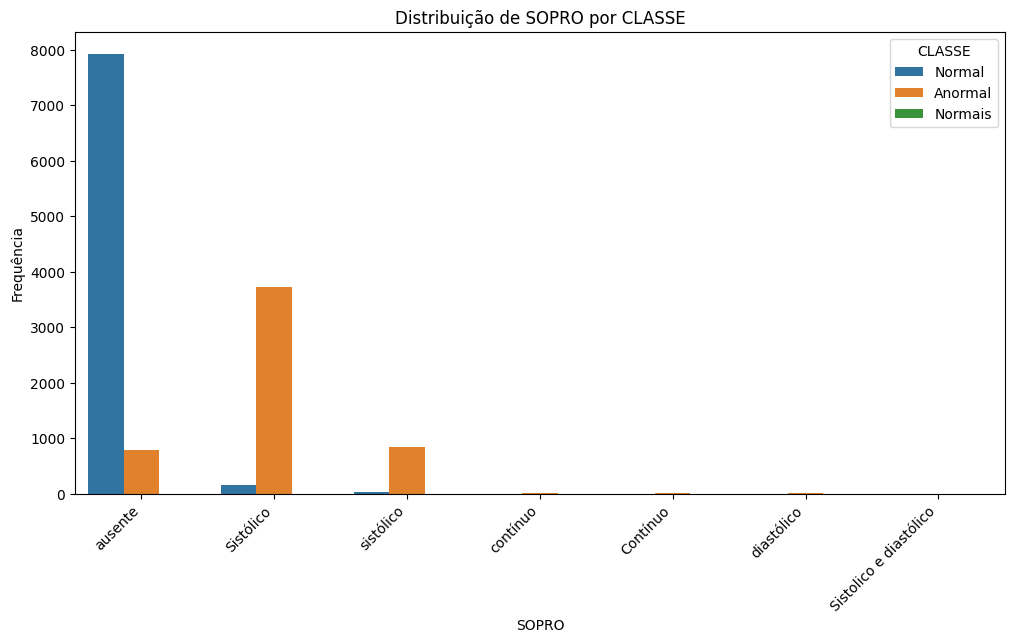
\includegraphics[width=\textwidth]{sopro.png}
    \tiny{\caption{Gráfico de sopro}}
    \label{fig:sopro}
  \end{minipage}
  \label{fig:exemplo}
\end{figure}

O atributo classe foi analisado por meio de um gráfico de pizza, que ilustra a distribuição das classes no conjunto de treinamento. 
A partir da visualização, observa-se que a proporção de amostras da classe Normal excede a da classe Anormal em 20\%. 
Essa disparidade pode levar a um viés no modelo, favorecendo a classe majoritária. Logo, é evidente a necessidade de remover uma 
certa quantidade de amostras pertencentes à classe Normal, visando evitar o viés.

\begin{figure}[htbp]
  \centering
  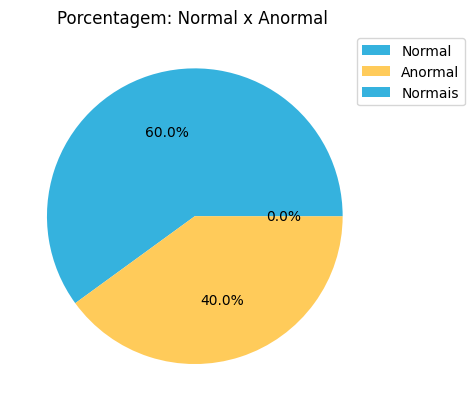
\includegraphics[width=0.15\textwidth]{distribuicao_classe.png}
  \tiny{\caption{distribuicao de classes no conjunto de treino}}
  \label{fig:classe}
\end{figure}


\subsection{Pré-processamento}
Devido ao número limitado de amostras no conjunto de treino, optou-se por preservar o máximo possível de dados, preferindo a imputação de valores nulos e irregulares nas colunas numéricas em vez de sua remoção. Primeiro, valores irreais foram definidos como nulos para não distorcer as medidas descritivas. Em seguida, aplicou-se a imputação pela mediana nos valores faltantes, após isso , o IMC foi recalculado com base nos novos valores. A mediana foi escolhida devido ao alto desvio padrão em relação à grandeza dos atributos.

\vspace{0.3cm}
\begin{center}
{\scriptsize
\begin{tabular}{|c|c|c|c|c|c|}
\hline 
Peso & Altura & IDADE & PA SISTOLICA & PA DIASTOLICA & FC \\ 
\hline
17.31   & 33.29   & 4.59 & 10.58 & 8.68 & 16.63   \\ 
\hline
\end{tabular}
}
\vspace{0.1cm}
\par {\scriptsize Valores do desvio padrão de cada atributo tratado.}
\end{center}
\vspace{0.2cm}


Para as colunas categóricas, a maioria das amostras com valores faltantes foi removida, exceto em "Pulsos", "HDA2", "MOTIVO2" e "PPA". Os três primeiros casos foram mantidos devido ao grande número de valores faltantes, cuja remoção prejudicaria o treinamento do modelo, enquanto "PPA" continha a categoria 'Não calculado', que foi usada para substituir os nulos.

No conjunto de testes, a abordagem foi similar, com a diferença de que todos os valores faltantes nas colunas categóricas foram substituídos pela moda, já que a remoção de amostras não era permitida.

Após o tratamento dos valores espúrios, criou-se o atributo 'SOPRO PESO', combinando 'SOPRO' e 'Peso'. A decisão foi motivada pela alta correlação do atributo target com ambos, além da forte correlação entre eles. Para evitar redundância, o atributo 'Peso' foi removido, já que sua informação foi incorporada no novo atributo.

As colunas numéricas foram normalizadas utilizando o método QuantileTransformer. Essa abordagem teve como objetivo reduzir o impacto de outliers no modelo e padronizar a escala dos valores, já que alguns algoritmos, como a Regressão Logística, são sensíveis a diferenças de grandeza entre os atributos.

As colunas categóricas foram mapeadas através do método One Hot Label Encoding, para evitar a criação de pesos ou hierarquias inadequadas aos valores.


\section{Protocolo experimental}
Neste projeto, foram implementados os seguintes modelos de aprendizado: K-Neighbors, Naive Bayes, Regressão Logística,
Redes neurais artificiais, Máquinas de vetores de suporte e floresta aleatória.
A técnica de florestas aleatórias foi escolhida pois a mesma mostrou bons resultados para diversos trabalhos relacionadoa à dados médicos.

Como modelos como florestas aleatórias, máquinas de vetores de suporte, redes neurais artificiais e regressão logística são sensíveis à alteração de seus hiper-parâmetros, foi utiliziado o método de GridSearch para encontrar os melhores parâmetros para cada um desses modelos. A busca foi feita utilizando o conjunto de treino utilizando cross-validation com 5 folds, onde a combinação que apresentou a melhor acurácia seria selecionada.
A  busca foi estruturada da seguinte forma:
\vspace{0.3cm}

\begin{itemize}
        \item Na regressão logística foram testados valores de C em um intervalo de 10\textsuperscript{-2} até 10\textsuperscript{3} com passo de 1 na potência.
        \item O número de hidden-layer-sizes para redes neurais artificiais foi testado em um intervalo de 10 até 40.
        \item No caso de máquinas de vetores de suporte com kernel linear, foram testados valores de C em um intervalo de 10\textsuperscript{-2} até 10\textsuperscript{3} com passo de 1 na potência.
        \item Para máquinas de vetores de suporte com kernel linear e com kernel polinomial, foram testados valores de \( C \) e \( \gamma \) em um intervalo de \( 10^{-2} \) até \( 10^{3} \) com passo de 1 na potência.

        \item O número de estimators em random forest foi testado em um intervalo de 100 a 300, com incremento de 50.
\end{itemize}

\vspace{0.3cm}
Após o término da busca, os seguintes valores de hiper-parâmetros foram escolhidos:

\vspace{0.3cm}
\begin{itemize}
    \item Regressão Logística: \( C = 1 \).
    \item Florestas aleatórias: 150 estimators.
    \item Redes Neurais Artificiais: 10 hidden layers.
    \item Máquinas de vetores de suporte (linear): \( C = 0.1 \).
    \item Máquinas de vetores de suporte (radial): \( C = 1, 
    \gamma = 0.1 \).
    \item Máquinas de vetores de suporte (polinomial): \( C = x, 
    \gamma = x \).
\end{itemize}

\vspace{0.3cm}

Todos os modelos, assim como os métodos de pré-processamento e avaliação, foram implementados utilizando a biblioteca scikit-learn.

Afim de obter os resultados avaliativos, foi utilizado o método cross-validation com 5 folds. Para avaliar os modelos, foram calculadas a média e desvio padrão de cada uma das seguintes medidas de avaliação:

\vspace{0.3cm}

\begin{itemize}
  \item Acurácia - Proporção de previsões corretas em relação ao total de previsões.
  \item Precisão - Proporção de verdadeiros positivos entre todas as previsões classificadas como positivas.
  \item Recall - Proporção de verdadeiros positivos identificados corretamente em relação a todos os casos positivos reais.
  \item F1 Score - Média harmônica entre precisão e recall, equilibrando os dois indicadores.
\end{itemize}

  \vspace{0.3cm}

  Adicionalmente, a curva ROC foi plotada a partir da divisão do conjunto de treinamento em 80\% para treino e 20\% \
  para teste. Essa análise visou identificar o modelo com o maior valor de AUC, permitindo selecionar a melhor opção para a competição 
  com base no desempenho discriminativo.



\section{Resultados}

\begin{table}[ht]
  \tiny
  \centering
  \begin{tabular}{l
                  S[table-format=2.2(2)]
                  S[table-format=2.2(2)]
                  S[table-format=2.2(2)]
                  S[table-format=1.2(2)]}
  \toprule
  \textbf{Modelo} & \textbf{Acurácia (\%)} & \textbf{Precisão (\%)} & \textbf{Recall (\%)} & \textbf{F1 Score (\%)} \\
  \midrule
  Random Forest       & 88.63 \pm 1.74 & 72.28 \pm 5.45 & 3.20 \pm 1.58 & 0.86 \pm 0.02 \\
  SVM Radial          & 87.83 \pm 2.10 & 72.17 \pm 6.17 & 4.34 \pm 1.59 & 0.85 \pm 0.03 \\
  SVM Polinomial      & 87.45 \pm 1.92 & 71.27 \pm 5.72 & 4.45 \pm 1.52 & 0.85 \pm 0.02 \\
  SVM Linear          & 87.33 \pm 2.12 & 70.51 \pm 5.74 & 4.25 \pm 1.84 & 0.85 \pm 0.02 \\
  Regressão Logística & 86.10 \pm 1.98 & 71.24 \pm 5.27 & 6.46 \pm 1.96 & 0.84 \pm 0.02 \\
  Redes Neurais       & 86.10 \pm 1.98 & 71.24 \pm 5.27 & 6.46 \pm 1.96 & 0.84 \pm 0.02 \\
  7-NN                & 85.67 \pm 1.99 & 76.96 \pm 5.11 & 5.73 \pm 2.17 & 0.83 \pm 0.03 \\
  5-NN                & 85.52 \pm 1.72 & 70.84 \pm 4.77 & 6.96 \pm 2.17 & 0.83 \pm 0.02 \\
  3-NN                & 84.07 \pm 2.87 & 71.75 \pm 5.53 & 9.77 \pm 3.10 & 0.82 \pm 0.03 \\
  Naïve Bayes         & 82.51 \pm 2.15 & 72.06 \pm 4.88 & 12.27 \pm 2.42 & 0.80 \pm 0.03 \\
  \bottomrule
  \end{tabular}
\end{table}

A tabela acima apresenta a média e desvio padrão de todas as medidas de desempenho selecionados, em ordem decrescente de acurácia.

A análise dos resultados demonstra que a maioria dos métodos avaliados foi eficaz na detecção de pacientes com condições cardíacas anormais, 
apresentando desempenho satisfatório em termos de precisão e recall. Observa-se que as técnicas de classificação conseguiram identificar corretamente 
uma proporção significativa de casos anormais, com destaque para métodos como Random Forest e máquinas de vetores de suporte (SVM) com diferentes kernels, que alcançaram um equilíbrio adequado entre a detecção de casos anormais e a minimização de falsos positivos.

No entanto, é crucial ressaltar que alguns métodos apresentaram taxas elevadas de classificação incorreta de pacientes saudáveis como anormais, o que pode comprometer sua aplicação em cenários clínicos reais. Nesse aspecto, técnicas como Random Forest e SVM com kernel polinomial se destacaram por apresentarem as menores taxas de falsos positivos, sendo consideradas mais adequadas para aplicações práticas.

Em termos de desempenho geral, o Random Forest obteve os melhores resultados, com um equilíbrio notável entre acurácia, precisão e recall. Métodos como regressão logística e SVM com kernels radial e linear também demonstraram resultados consistentes, embora ligeiramente inferiores. Por outro lado, técnicas baseadas em k-NN e Naive Bayes apresentaram desempenho menos satisfatório, principalmente devido às taxas mais altas de classificação incorreta de pacientes saudáveis.


Os desempenhos obtidos no public leaderboard da competição do Kaggle demonstraram consistência e robustez, com as acurácias variando entre 93,7\% 
e 93,8\%. Esses resultados refletem não apenas a alta capacidade de generalização dos modelos desenvolvidos, mas também a eficácia das técnicas 
empregadas na tarefa de classificação. A proximidade entre as métricas alcançadas indica que os modelos mantiveram um equilíbrio entre precisão e recall, 
garantindo uma detecção confiável de casos anormais sem comprometer significativamente a taxa de falsos positivos.


\section{Estratégia final}


Para determinar quais modelos seriam utilizados na competição, realizou-se a plotagem das curvas ROC e o cálculo dos respectivos valores de AUC 
(Área Sob a Curva), utilizando um conjunto de 80\% treino e 20\% teste. Como a métrica de avaliação da competição era baseada no valor de AUC, optou-se por selecionar os dois modelos que apresentaram os 
maiores valores dessa métrica, garantindo assim um desempenho superior na classificação. Após a análise das curvas ROC e dos cálculos, os valores de AUC 
obtidos para cada modelo foram organizados e estão apresentados na tabela abaixo. 

\vspace{0.3cm}
\begin{center}
{\scriptsize
\begin{tabular}{|c|c|}
\hline 
Modelo & AUC \\ 
\hline
Random Forest & 95.98\% \\ 
\hline
Regressão Logística & 95.51\% \\ 
\hline
Redes Neurais & 95.42\%  \\ 
\hline
SVM radial & 95.11\% \\ 
\hline
7-NN & 94.64\% \\ 
\hline
SVM polinomial & 94.56\% \\ 
\hline
5-NN & 94.36\% \\ 
\hline
3-NN & 94.36\% \\ 
\hline
Naive Bayes & 94.16\% \\ 
\hline
SVM linear & 93.28\% \\ 
\hline
\end{tabular}
}
\vspace{0.1cm}
\par {\scriptsize AUC de cada modelo}
\end{center}
\vspace{0.2cm}

Com base na análise das curvas ROC e nos valores de AUC, os modelos selecionados para a competição foram o Random Forest, 
com 150 estimators, e a Regressão Logística, com o parâmetro de regularização C=1. Esses modelos se destacaram por apresentarem os maiores valores de 
AUC, demonstrando alta capacidade de distinção entre as classes e um desempenho superior na tarefa de classificação. 


\begin{figure}[htbp]
  \centering
  \begin{minipage}{0.2\textwidth} 
    \centering
    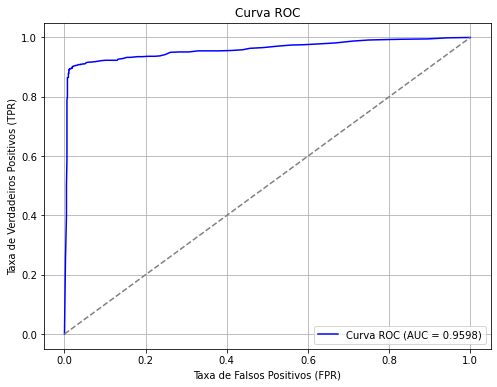
\includegraphics[width=\textwidth]{roc_rf.png} 
    \tiny{\caption{Curva ROC do modelo random forest}}
    \label{fig:Curva ROC do modelo random forest}
  \end{minipage}
  \hfill 
  \begin{minipage}{0.2\textwidth}
    \centering
    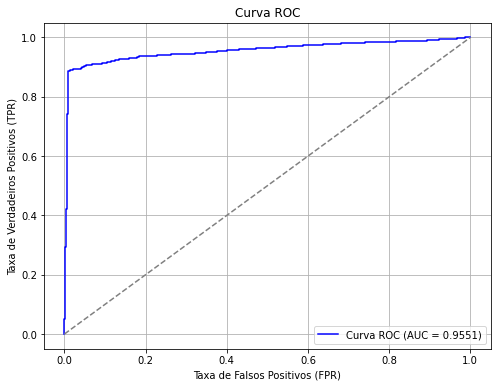
\includegraphics[width=\textwidth]{roc_rl.png}
    \tiny{\caption{Curva ROC do modelo regressão logística}}
    \label{fig:Curva ROC do modelo regressão logística}
  \end{minipage}
  \label{fig:exemplo}
\end{figure}

\section{Conclusões}

Este trabalho teve como objetivo desenvolver um sistema para a detecção precoce de patologias cardiovasculares em pacientes pediátricos, empregando diversas técnicas de aprendizado de máquina. 

Os resultados obtidos demonstram que os métodos de classificação avaliados foram eficazes na detecção de pacientes com condições cardíacas anormais, garantindo um bom equilíbrio entre precisão e recall. Em especial, o Random Forest se destacou por apresentar um desempenho robusto, conciliando alta acurácia com uma baixa taxa de falsos positivos. Modelos como SVM com kernel polinomial e regressão logística também mostraram resultados consistentes, reforçando sua viabilidade para aplicações clínicas.

No entanto, algumas técnicas apresentaram limitações, como o k-NN e o Naive Bayes, que tiveram dificuldades na correta classificação de pacientes saudáveis, resultando em um número elevado de falsos positivos. Esse fator ressalta a importância da escolha criteriosa do modelo para garantir um diagnóstico mais confiável.

Como sugestão de extensão para o trabalho, é interessante a ampliação do conjunto de dados por meio da inclusão de atributos clínicos mais detalhados, especialmente aqueles diretamente relacionados à saúde cardiovascular.
\begin{thebibliography}{1}

  \bibitem{IEEEhowto:kopka}
  Aprendizado de Máquina para
Predição de Diagnósticos de Doenças Cardiovasculares, Fran-
cisco Romes da Silva Filho e Emanuel F. Coutinho.(2022)

\bibitem{citekey}
Ghosh, P., Azam, S., Jonkman, M., Karim, A., Shamrat, F. M. J. M., Ignatious, E., Shul-
tana, S., Beeravolu, A. R., and De Boer, F. (2021). Efficient prediction of cardiovas-
cular disease using machine learning algorithms with relief and lasso feature selection
techniques. 

    
  
  \end{thebibliography}

\end{document}

% For peer review papers, you can put extra information on the cover
% page as needed:
% \ifCLASSOPTIONpeerreview
% \begin{center} \bfseries EDICS Category: 3-BBND \end{center}
% \fi
%
% For peerreview papers, this IEEEtran command inserts a page break and
% creates the second title. It will be ignored for other modes.
\IEEEpeerreviewmaketitle



\section{Introduction}
% no \IEEEPARstart
This demo file is intended to serve as a ``starter file''
for IEEE conference papers produced under \LaTeX\ using
IEEEtran.cls version 1.7 and later.

All manuscripts must be in English. These guidelines include complete descriptions of the fonts, spacing, and related information for producing your proceedings manuscripts. Please follow them and if you have any questions, direct them to the production editor in charge of your proceedings at Conference Publishing Services (CPS): Phone +1 (714) 821-8380 or Fax +1 (714) 761-1784.
% You must have at least 2 lines in the paragraph with the drop letter
% (should never be an issue)

\subsection{Subsection Heading Here}
Subsection text here.


\subsubsection{Subsubsection Heading Here}
Subsubsection text here.

\section{Type style and Fonts}
Wherever Times is specified, Times Roman or Times New Roman may be used. If neither is available on your system, please use the font closest in appearance to Times. Avoid using bit-mapped fonts if possible. True-Type 1 or Open Type fonts are preferred. Please embed symbol fonts, as well, for math, etc.


% An example of a floating figure using the graphicx package.
% Note that \label must occur AFTER (or within) \caption.
% For figures, \caption should occur after the \includegraphics.
% Note that IEEEtran v1.7 and later has special internal code that
% is designed to preserve the operation of \label within \caption
% even when the captionsoff option is in effect. However, because
% of issues like this, it may be the safest practice to put all your
% \label just after \caption rather than within \caption{}.
%
% Reminder: the "draftcls" or "draftclsnofoot", not "draft", class
% option should be used if it is desired that the figures are to be
% displayed while in draft mode.
%
%\begin{figure}[!t]
%\centering
%\includegraphics[width=2.5in]{myfigure}
% where an .eps filename suffix will be assumed under latex, 
% and a .pdf suffix will be assumed for pdflatex; or what has been declared
% via \DeclareGraphicsExtensions.
%\caption{Simulation Results}
%\label{fig_sim}
%\end{figure}

% Note that IEEE typically puts floats only at the top, even when this
% results in a large percentage of a column being occupied by floats.


% An example of a double column floating figure using two subfigures.
% (The subfig.sty package must be loaded for this to work.)
% The subfigure \label commands are set within each subfloat command, the
% \label for the overall figure must come after \caption.
% \hfil must be used as a separator to get equal spacing.
% The subfigure.sty package works much the same way, except \subfigure is
% used instead of \subfloat.
%
%\begin{figure*}[!t]
%\centerline{\subfloat[Case I]\includegraphics[width=2.5in]{subfigcase1}%
%\label{fig_first_case}}
%\hfil
%\subfloat[Case II]{\includegraphics[width=2.5in]{subfigcase2}%
%\label{fig_second_case}}}
%\caption{Simulation results}
%\label{fig_sim}
%\end{figure*}
%
% Note that often IEEE papers with subfigures do not employ subfigure
% captions (using the optional argument to \subfloat), but instead will
% reference/describe all of them (a), (b), etc., within the main caption.


% An example of a floating table. Note that, for IEEE style tables, the 
% \caption command should come BEFORE the table. Table text will default to
% \footnotesize as IEEE normally uses this smaller font for tables.
% The \label must come after \caption as always.
%
%\begin{table}[!t]
%% increase table row spacing, adjust to taste
%\renewcommand{\arraystretch}{1.3}
% if using array.sty, it might be a good idea to tweak the value of
% \extrarowheight as needed to properly center the text within the cells
%\caption{An Example of a Table}
%\label{table_example}
%\centering
%% Some packages, such as MDW tools, offer better commands for making tables
%% than the plain LaTeX2e tabular which is used here.
%\begin{tabular}{|c||c|}
%\hline
%One & Two\\
%\hline
%Three & Four\\
%\hline
%\end{tabular}
%\end{table}


% Note that IEEE does not put floats in the very first column - or typically
% anywhere on the first page for that matter. Also, in-text middle ("here")
% positioning is not used. Most IEEE journals/conferences use top floats
% exclusively. Note that, LaTeX2e, unlike IEEE journals/conferences, places
% footnotes above bottom floats. This can be corrected via the \fnbelowfloat
% command of the stfloats package.



\section{Conclusion}
The conclusion goes here. this is more of the conclusion

% conference papers do not normally have an appendix


% use section* for acknowledgement
\section*{Acknowledgment}


The authors would like to thank...
more thanks here


% trigger a \newpage just before the given reference
% number - used to balance the columns on the last page
% adjust value as needed - may need to be readjusted if
% the document is modified later
%\IEEEtriggeratref{8}
% The "triggered" command can be changed if desired:
%\IEEEtriggercmd{\enlargethispage{-5in}}

% references section

% can use a bibliography generated by BibTeX as a .bbl file
% BibTeX documentation can be easily obtained at:
% http://www.ctan.org/tex-archive/biblio/bibtex/contrib/doc/
% The IEEEtran BibTeX style support page is at:
% http://www.michaelshell.org/tex/ieeetran/bibtex/
%\bibliographystyle{IEEEtran}
% argument is your BibTeX string definitions and bibliography database(s)
%\bibliography{IEEEabrv,../bib/paper}
%
% <OR> manually copy in the resultant .bbl file
% set second argument of \begin to the number of references
% (used to reserve space for the reference number labels box)
\begin{thebibliography}{1}

\bibitem{IEEEhowto:kopka}
H.~Kopka and P.~W. Daly, \emph{A Guide to \LaTeX}, 3rd~ed.\hskip 1em plus
  0.5em minus 0.4em\relax Harlow, England: Addison-Wesley, 1999.

\bibitem{citekey}
As consequências da DCV. Ghosh et al. (2021)

\end{thebibliography}




% that's all folks
\end{document}


